\chapter{Meetresultaten}%
\label{ch:benchmarks}

De performantie van WebGPU in vergelijking met andere technologieën kan sterk verschillen. Om eem beeld te vormen voor over de capaciteiten die \textit{WebGPU} brengt op de browser worden in dit hoofdstuk enkele testen uitgevoerd. Hierdoor kan er vergeleken worden hoe de prestaties van \textit{WebGPU} al dan niet overeenstemmen met traditionele technologieën zoals \textit{CUDA}.

\bigbreak{}

Om gebruik te maken van \textit{GPU} acceleratie, is het vereist dat applicaties communiceren met een \textit{GPU application programming interfaces (APIs)}. Zo bestaan er onderliggend in besturingssystemen \textit{APIs} zoals Direct3D 12 voor Microsoft Windows, Metal voor ontwikkeling op het Apple ecosysteem en Vulcan als open standaard. Dit zijn complexe software oplossingen die de beste prestaties bieden en hierdoor toelaten dat software optimaal gebruik kan maken van de onderliggende \textit{hardware}. Deze grafische APIs zorgen telkens voor de communicatie tussen applicaties en de onderliggende grafische computeronderdelen. En laten dus voor computationeel complexe programma's toe om parallelle berekeningen uit te voeren op krachtige grafische kaarten.

\bigbreak{}

Het is echter duidelijk dat het onderhouden van software voor verschillende besturingssystemen complex is en veel energie vergt, dit zorgt ervoor dat applicaties vaak maar beperkt worden ondersteund. Dit is een probleem dat WebGPU verhelpt door een abstractie laag te vormen boven deze APIs. \autocite{Wallez2023} 

\break{}

\section{Transformer prestaties van WASM en WebGPU}

Een andere opkomende technologie is  \textit{web assembly} (WASM). WASM is een zeer compact \textit{assembly-like binary} die performantie toelaat vergelijkbaar met \textit{native} talen zoals C/C++ en Rust. \autocite{Steiner2023} 

\bigbreak{}

Deze \textit{low-level} programmeer talen laten net zoals \textit{WGSL} voor \textit{WebGPU} toe dat rekenkundige taken optimaal worden uitgevoerd. Dit komt omdat code specifiek wordt geschreven op een manier die rekening houdt met hoe de onderliggende hardware functioneert.

\bigbreak{}

\pgfplotsset{width=15cm,compat=1.9}

% We will externalize the figures
% \tikzexternalize
\pgfplotsset{
  log ticks with fixed point,
}
\begin{tikzpicture}
    \begin{semilogxaxis}[
        title={Transformer benchmark fp32 WASM versus WebGPU},
        xlabel={Batch size},
        ylabel={Execution time in ms},
        xmin=1, xmax=64,
        ymin=0, ymax=70000,
        xtick={1,2,4,8,16,32, 64},
        ytick={1,10000,20000,30000,400000,50000,60000, 70000},
        legend pos=north west,
        ymajorgrids=true,
        grid style=dashed,
        scatter/classes={
            a={mark=square*,red},
            b={mark=triangle*,orange},
            c={mark=o,draw=blue},
            d={mark=square,green}
        },
        yticklabel style={
            /pgf/number format/fixed,
        },
        scaled y ticks=false
    ]
    
    \addplot[
        color=red,
        mark=square*
        ]
        coordinates {
            (1, 946.14)(2, 1923.12)(4, 3816.90)(8, 7653.00)(16, 15494.62)(32, 30901.40)(64, 61788.00)
        };
        \addlegendentry{WASM (fp32) Intel Xeon E5-2680 V2}
        
    \addplot[
        color=orange,
        mark=triangle*
        ]
        coordinates {
            (1, 747.10)(2, 1499.98)(4, 3014.38)(8, 5956.38)(16, 11807.70)(32, 24121.56)(64, 47769.14)
        };
        \addlegendentry{WASM (fp32) Intel Core i9-9980HK}
    \addplot[
        color=blue,
        mark=o
        ]
        coordinates {
            (1, 193.66)(2, 365.90)(4, 703.24)(8, 1393.12)(16, 2752.66)(32, 5510.74)(64, 10966.04)
        };
        \addlegendentry{WebGPU (fp32) Intel UHD Graphics 630}

    \addplot[
        color=green,
        mark=square
        ]
        coordinates {
            (1, 28.02)(2, 58.28)(4, 77.74)(8, 116.40)(16, 226.00)(32, 463.16)(64, 739.16)
        };
        \addlegendentry{WebGPU (fp32) Nvidia Geforce GTX 1080 Ti}
    \addplot [
        scatter,only marks,
        scatter src=explicit symbolic,
    ] table [x=x,y=y,meta=label] {plotdata/HuggingFaceWasmVSWebGPU.dat};

    \end{semilogxaxis}
\end{tikzpicture}

Door de \textit{webgpu-embedding-benchmark} van \textcite{Lochner2024} uit te voeren met verschillende test-opstellingen blijkt WebGPU consistent sneller dan WASM. In deze test werd de uitvoeringstijd gemeten van \textit{BERT-based embedding} modellen met zowel WebGPU als WASM, en dit telkens voor een toenemende \textit{batch size}.

\break{}

\begin{tabular}{ |p{5cm}|p{3cm}|p{3cm}|p{3cm}|  }
    \hline
    \multicolumn{4}{|c|}{Vergelijken van theoretische \textit{Floating Point} performantie} \\
    \hline
    Component& Theoretisch GFLOPS & Theoretisch baseline & Meetresultaten WASM WebGPU\\
    \hline
        Xeon E5-2680 V2             & 224,0     & 100\%  & 100\%       \\
        Intel Core i9-9980HK        & 307,2     & 137\%  & 129\%    \\
        Intel UHD Graphics 630      & 403,2     & 180\%  & 560\%    \\
        Nvidia Geforce GTX 1080 Ti  & 11.340,0  & 5063\% & 7170\%   \\
    \hline
\end{tabular}

\bigbreak{}

Voor een \textit{batch-size} van 64 doet de \textit{Xeon E5-2680 V2} gemiddeld 60s over de transformer test. Wanneer deze tijd als basis wordt genomen is de Intel Core i9-9980HK 10 seconden sneller.

\bigbreak{}

De \textit{Xeon E5-2680 V2} werd als basis gebruikt om de andere componenten te vergelijken. Omdat de \textit{Intel Core i9-9980HK} een nieuwere processor is, is deze gemiddeld voor alle \textit{batch} groottes 30\% sneller. Voor beide deze processoren werd de Intel specificatie gebruikt om de theoretische \textit{GFLOPS} te bepalen. \autocite{Intel2024, Intel2024a}

\bigbreak{}

De \textit{GFLOPS} voor de grafische kaarten werd gebaseerd op informatie die beschikbaar werd gesteld door \textcite{TechPowerUp2017, TechPowerUp2017a}.

\bigbreak{}

Uit de grafiek en de tabel valt af te leiden dat voor deze test WebGPU beter presteert dan WASM. Deze test toont enkel resultaten die vergelijkbaar zijn wanneer kunstmatige intelligentie modellen getraind worden vanuit de browser. Deze test is niet representatief voor alle scenario's, zoals bijvoorbeeld het operationeel draaien van een model.

\bigbreak{}

Ook valt af te leiden uit de resultaten van de \textit{webgpu-embedding-benchmark} van \textcite{Lochner2024} dat WebGPU beter presteert dan verwacht uit de theoretische snelheden. Dit ligt aan de implementatie van de test. Net zoals \textit{WebGPU} is \textit{WebAssembly} een nieuwe technologie. Beide technologieën zijn nog in ontwikkeling en kunnen nog verder verbeterd worden om de prestaties te verhogen. 

\bigbreak{}

Zowel theoretische waarden als meetresultaten werden telkens vergeleken met de \textit{base line} gebaseerd op de performantie van de \textit{Xeon E5-2680 V2}. Bij het uitvoeren van deze testen werd de sequentie lengte ingesteld op 512 en alle testen werden uitgevoerd met \emph{Chrome 124.0.6367.93}.

\break{}

\section{Grafische capaciteiten WebGL, WebGL 2.0 en WebGPU}

Grafische rendering op het web werd sinds 2011 afgehandeld door \textit{WebGL}. Deze technologie is echter verouderd en werd vervangen met \textit{WebGL 2.0} in 2017. Sinds \textit{WebGL 2.0} zijn er nieuwe grafische technologieën op de markt zoals \textit{ray tracing}, waarbij individuele fotonen worden gesimuleerd om extreem realistische belichting te simuleren. Deze nieuwe technologieën werden niet verwerkt in WebGL maar worden wel verwacht in WebGPU.

\bigbreak{}

Het is dus belangrijk te vermelden dat \textit{WebGPU} niet enkel vernieuwingen brengt in de vorm van algemene rekenkracht, maar ook de grafische prestaties verschillen tussen \textit{WebGL 2.0} en \textit{WebGPU}. 

\bigbreak{}

Deze bewering kan getest worden aan de hand van enkele voorbeelden

\break{}

\section{Whisper implementaties met CPU, CUDA en WebGPU}

Omdat de AI-modellen van Whisper online worden gepubliceerd door \textcite{OpenAI2023}; laat dit toe de vergelijking te maken tussen verschillende implementaties van deze AI-modellen. Deze kunnen namelijk normaal met een CPU worden gebruikt maar ook met \textit{CUDA} en WebGPU. Deze laatste is mogelijk omwille van de implementaties van \textcite{Fleetwood2024, Fleetwood2023b}.

\bigbreak{}

De modellen van OpenAI met verschillende parameter groottes zijn beschikbaar op \href{https://github.com/openai/whisper}{GitHub.com/OpenAI/Whisper}.

\bigbreak{}

\begin{table}
    \begin{tabular}{ |p{1.5cm}|p{2.5cm}|p{3cm}|p{3cm}|p{2cm}|p{2cm}|  }
        \hline
        \multicolumn{6}{|c|}{Beschikbare modellen en talen Whisper} \\
        \hline
            Size& Parameters & English-only model & Multilingual model & Required VRAM & Relative speed\\
        \hline
            tiny&       39 M    &tiny.en    & tiny& ~1 GB& ~32x     \\
            base &      74 M	&base.en    & base & ~1 GB & ~16x   \\
            small &     244 M	&small.en   & small & ~2 GB & ~6x   \\
            medium &    769 M	&medium.en  & medium & ~5 GB & ~2x  \\
            large &     1550 M	&N/A        & large & ~10 GB& 	1x  \\
        \hline
    \end{tabular}
    \caption{Whisper modellen beschikbaar gesteld door \textcite{OpenAI2023}.}
    \label{tab:OpenAIWhisperModels}
\end{table}

\bigbreak{}

Juist omdat Whisper zoveel verschillende model groottes beschikbaar stelt maakt dit AI-model zeer geschikt om te testen met WebGPU, maar ook met CUDA en normale processor implementaties. Door verschillende grafische kaarten en processoren te testen kon hierdoor een beeld gegeven worden wat de verwacht prestaties zijn die WebGPU kan bieden in vergelijking met normale processor implementaties, of geavanceerdere CUDA implementaties.

\bigbreak{}

Om testresultaten op een consistente manier te verzamelen werd een python script geschreven. Dit script werd dan op verschillende apparaten uitgevoerd om op deze manier betrouwbare data te verzamelen. Dit script kan in detail bekeken worden in de bijlage.

\bigbreak{}

Om de prestaties van WebGPU te onderzoeken werd de implementatie van \textcite{Fleetwood2024} gebruikt. Deze logt namelijk telkens de inferentie tijd die nodig was voor het uitvoeren. Deze data moet manueel verzameld worden.

\bigbreak{}

\subsection*{Installatie afhankelijkheden}

Om Whisper werkende te krijgen op een \textit{Windows 10} installatie zijn er verschillende afhankelijkheden die moeten worden geïnstalleerd. Dit betreft \textit{Python 3.9.9}, \textit{PyTorch 1.10.1} en de \textit{CUDA toolkit}. Het is ook belangrijk op te merken dat Torch moet worden gecompileerd met \textit{CUDA} functionaliteit, indien dit niet wordt gedaan kan enkel de CPU geaccelereerd versie van het Whisper model worden uitgevoerd.

\bigbreak{}

% PS > pip3 uninstall torch torchvision==0.15.0 torchaudio==2.0.0
% PS > pip3 cache purge
% PS > pip3 install torch torchvision==0.15.0 torchaudio==2.0.0 --index-url https://download.pytorch.org/whl/cu117

\begin{lstlisting}[language=python]
import torch
torch.cuda.is_available()
# returns False
torch.zeros(1).cuda()
# throws AssertionError: Torch not compiled with CUDA enabled
\end{lstlisting}

% \begin{lstlisting}[language=python]
% import torch
% torch.cuda.is_available()
% # returns True
% torch.zeros(1).cuda()
% # returns tensor([0.], device='cuda:0')
% \end{lstlisting}

\pgfplotsset{width=12cm,compat=1.9}

\pgfplotsset{
  log ticks with fixed point,
}

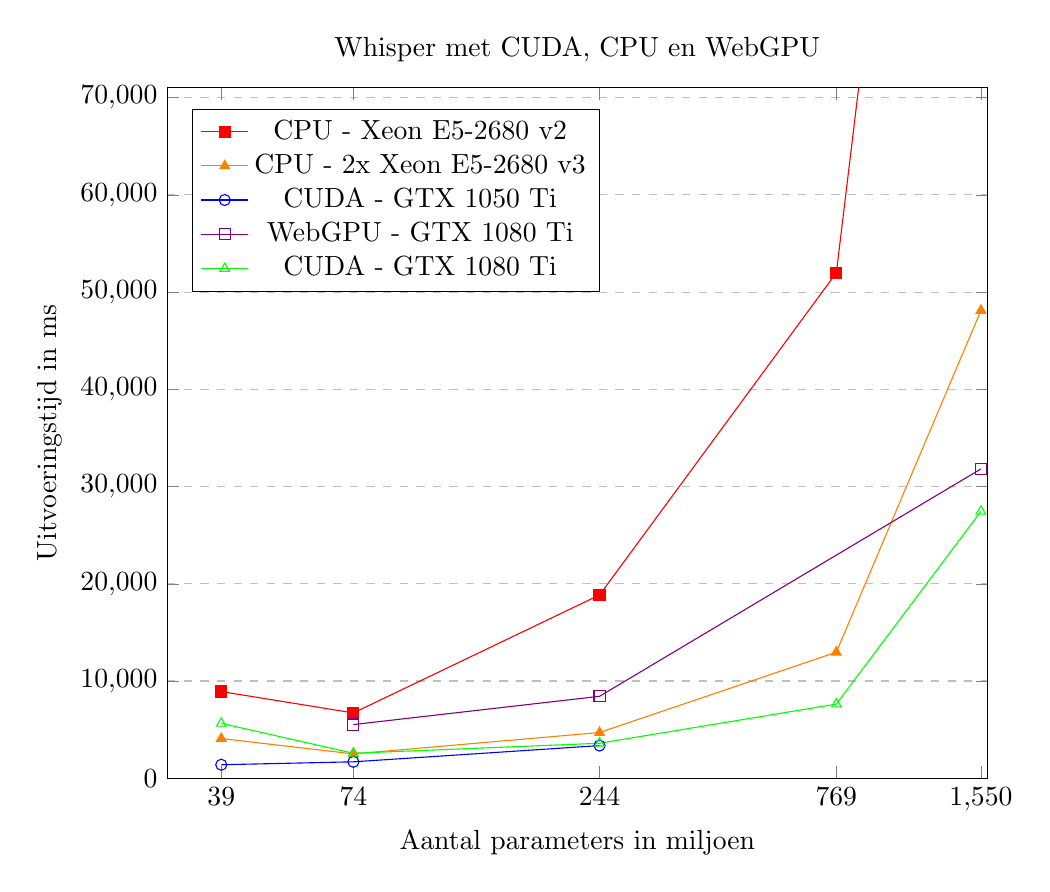
\begin{tikzpicture}
    \begin{semilogxaxis}[
        title={Whisper met CUDA, CPU en WebGPU},
        xlabel={Aantal parameters in miljoen},
        ylabel={Uitvoeringstijd in ms},
        xmin=30, xmax=1600,
        ymin=0, ymax=71000,
        xtick={39, 74, 244, 769, 1550},
        legend pos=north west,
        ymajorgrids=true,
        grid style=dashed,
        yticklabel style={
            /pgf/number format/fixed,
        },
        scaled y ticks=false
    ]
    \addplot[
            color=red,
            mark=square*
        ]
        coordinates {(39,8919)(74,6721)(244,18849)(769,51980)(1550,175378)};
        \addlegendentry{CPU - Xeon E5-2680 v2}
    \addplot[
        color=orange,
        mark=triangle*
        ]
        coordinates {(39,4088)(74,2508)(244,4706)(769,12963)(1550,48107)};
        \addlegendentry{CPU - 2x Xeon E5-2680 v3}
    \addplot[
            color=blue,
            mark=o
        ]
        coordinates {(39,1393)(74,1694)(244,3362)};
        \addlegendentry{CUDA - GTX 1050 Ti}
    \addplot[
            color=violet,
            mark=square
        ]
        coordinates {(74,5526)(244,8431)(1550,31814)};
        \addlegendentry{WebGPU - GTX 1080 Ti}
    \addplot[
            color=green,
            mark=triangle
        ]
        coordinates {(39,5647)(74,2574)(244,3602)(769,7629)(1550,27448)};
        \addlegendentry{CUDA - GTX 1080 Ti}
    \end{semilogxaxis}
\end{tikzpicture}

% pip3 install torch torchvision==0.15.0 torchaudio==2.0.0 --index-url https://download.pytorch.org/whl/cu117
% pip3 install torch torchvision==0.15.0 torchaudio==2.0.0 --index-url https://download.pytorch.org/whl/cpu
% pip3 uninstall torch torchvision==0.15.0 torchaudio==2.0.0
% pip3 cache purge

\section*{Opetten van de test}

Zodat er consistente relustaten konden worden geproduceerd uit de testen werd de test steeds op dezelfde test opstelling getest, hierbij werd Python code gebruikt om de Whisper implementatie met zowel Pytorch ondersteund door CUDA als Pytorch ondersteund door de rekenkracht van de processor.

\section*{Resultaten Whisper test}

\section{wgpu-bench}

Om de performantie te testen van WebGPU werd wgpu-bench uitgevoerd.

Hiervoor werd rust geïnstalleerd, en gebruik gemaakt van Visual Studio Community 2022 in combinatie met Visual Studio Build-Tools 2022, waarbij de \textit{Desktop development with C++} module werd meegeïnstalleerd.

De broncode moest hierna gebouwd worden.

% rustup default nightly-x86_64-pc-windows-msvc

\break{}
